\chapter{Vizualizační knihovna a rozšíření}\label{sec:Implementation2}

Tato část aplikace se zabývá, knihovnou určenou pro vizualizaci průchodů regulárními výrazy a rozšířením do vývojového prostředí \textit{VSCode}.
Pro získání informací o vyhledávání, slouží již zmíněná knihovna, která byla popsána v předchozí kapitole~\ref{sec:Implementation1}.
Hlavním cílem této části aplikace je, na implementovat uživatelsky přívětivé a intuitivní rozhraní, integrované do vývojového prostředí.
To umožňuje zadávat regulární výrazy, text ve kterém lze pomocí zadaného výrazu vyhledávat a následnou vizualizaci ve formě debuggeru.
Vizualizace je koncipována, jako webová stránka, která je zobrazená do prostředí pomocí tzv. webview, ale také může existovat samostatně.

\section{Návrh vizualizační části}

Vstupním souborem knihovny je HTML soubor \textit{main.html}.
Ten také vkládá skript \textit{index.ts}, jehož hlavním účelem je inicializovat vše potřebné pro chod aplikace.
Hlavní třídou, která se stará o obsluhu vizualizace je \textbf{RegexVisualizer}. 
Jejím úkolem je obsluhovat ostatní komponenty a přímo komunikuje s třídou \textit{Regexer}, ze které následně získává data pro vizualizaci.
Pro interakci uživatele slouží dva textové editory, ty jsou ve formě dvou tříd \textit{RegexEditor} a \textit{StringMatchEditor}.
Obsluhují HTML elementy pro zadávání textu, jejich základní funkcionalita je děděna ze třídy \textit{TextEditor}.
Pro samotnou vizualizaci ve formě ladícího nástroje, existuje třída \textit{RegexDebugger}.
Má za úkol, obsluhovat okno aplikace, kde se samotný debugger nachází.
Obsahuje i vlastní posuvník (\textit{Slider}), který dokáže vyvolávat události, obsahující informace o aktuální hodnotě posuvníku.
Také například disponuje možností automatického přehrávání a změnou rychlosti.

\section{Implementace textových editorů}

Ve vizualizaci se nachází dva textové editory.
První slouží pro zadávání regulárního výrazu a druhý pro zadávání řetězce, ve kterém proběhne vyhledávání, na základě zadaného výrazu.
Jejich funkcionalita je obalena ve dvou třídách, každá sloužící pro jiný textový editor a obě dědí ze třídy \textit{TextEditor}.
Tento vztah lze vidět na obrázku~\ref{fig:TextEditor}.

\begin{figure}[!h]
	\centering
	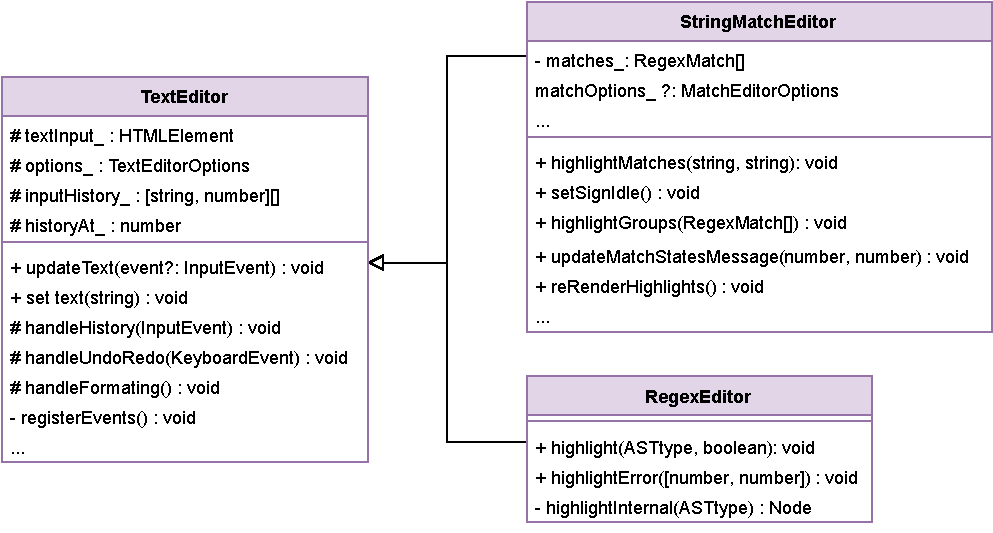
\includegraphics[width=0.8\textwidth]{Figures/TextEditor.pdf}
	\caption{Třídní diagram textových editorů}
	\label{fig:TextEditor}
\end{figure} 

\subsection*{Základní řešení}

Pro řešení textových editorů, jsem se rozhodl pro vlastní implementaci, pro větší flexibilitu a řešení konkrétních problému týkajících se práce s regulárními výrazy.
Textový editor umožňuje rozšířené možnosti práce s textem oproti HTML elementům, jako jsou input nebo textarea.
Tyto možnosti jsou například vlastní formátování, nebo správa historie. 
K realizaci samotných vstupů, jsem použil základní obalující HTML blok span.
Na zvoleném bloku tolik nezáleží, ale je potřeba, aby měl atribut \textit{contenteditable} s nastavenou hodnotou na true.
Tento atribut povoluje psaní přímo do daného bloku. 
Oproti elementu jako je input, lze zde vkládat HTML kód a tím upravovat formátování textu.
To je vhodné pro regulární výrazy, jelikož sami o sobě nejsou moc přehledné.

\textit{TextEditor} slouží jako vzorová třída, pro realizaci textových editorů.
Drží si referenci na HTML element, který obsluhuje, pod názvem \textit{textInput\_}. 
Pro lepší interaktivitu s tímto elementem, je potřeba zaregistrovat různé události.
Mezi ně patří např. psaní, mazání, undo a redo. 
Události jsou registrovány při vytvoření instance třídy, pomocí soukromé metody \textit{registerEvents}.
Pokud je zavolána, chráněná metoda \textit{handleFormating}, tak dojde ke změně podoby textu na formátovanou.
Jedná se o grafické zobrazení bílých znaků, jako je nový řádek nebo tabulátor.

\subsection*{Komunikace s třídou Regexer}

Komunikace funguje pomocí vyvolání událostí z textových editorů.
Je-li událost vyvolána editorem pro regulární výraz, tak se pomocí třídy \textit{Regexer} zpracuje daný výraz.
Pokud dojde k vyvolání události změny textu v jednom ze dvou editorů, tak dojde k zavolání metody pro vyhledávání (match).

Vyhledávání pak funguje na bázi asynchronní komunikace, kdy se výsledky posílají po tzv. dávkách (anglicky batch).
Výhodou této komunikace je to, že pokud uživatel v průběhu zpracovávání změní text jednoho z editorů, tak se proces ukončí a tím pádem není potřeba čekat na jeho dokončení.
Velikost jedné dávky jsem zvolil na 20000 stavů, jelikož tento počet stavů, je poměrně rychle vyhodnocený.
Informace o zpracování, se aktualizují průběžně po každé příchozí dávce.

\subsection*{Zvýraznění syntaxe}

Součástí třídy \textit{RegexEditor}, je metoda sloužící pro zvýrazňování syntaxe regulárních výrazů. 
Pro zvýraznění slouží získaná AST struktura po dokončeném parsování.
Algoritmus řešení tohoto problému, funguje na principu rekurzivního zanoření, ve stromové struktuře.
Každý symbol, který má být zvýrazněný je obalený v HTML bloku, s třídou identifikující o jaký symbol se jedná.
U některých vzorů, záleží na pořadí zpracování symbolů a rekurzivního zanoření.
Například skupina se zpracovává tak, že první se zvýrazní otevírací závorka "(".
Poté se algoritmus rekurzivně zanoří, nebo-li zpracuje potomky (vnitřní část) skupiny a nakonec zvýrazní ukončující závorku ")".
Výsledkem vznikne HTML struktura, která popisuje symboly a vzory regulárních výrazů.
Tyto symboly jsou pak zvýrazněny pomocí různých barev definovaných v CSS.

\subsection*{Historie}
Implementace historie textových editorů je vlastní, jelikož původní nefungovala správně.
Důvodem bylo časté přepisování textu, z již zmíněného formátování.
Aby historie správně fungovala, tak jsem musel vytvořit pole, které obsahuje jak původní řetězec tak pozici kurzoru v něm.
Pokud je vyvolána operace vrácení se zpět v historii (undo), překopíruje se uložený řetězec do textového pole a kurzor se nastaví na správnou pozici.
K odstranění záznamu z historie nedochází, jelikož může být vyvolána operace \textit{redo}, nebo-li odvolání operace \textit{undo}.
Pokud dojde k uložení nového stavu textového pole, tak všechny stavy za ukazatelem se smažou a přidá se zde nový.
V nastavení editoru, jsem přidal možnost zvolit si maximální počet záznamů v historii.
Pokud ale není nastavená, automaticky se omezí na 100 záznamů.

\subsection*{Pozice textového kurzoru}
Práce s textovým kurzorem je další značná část textových editorů.
Pokud uživatel píše do textového pole, tak často nastává změna textu na pozadí samotnou aplikací.
Například při zvýraznění, dochází ke změně textové formy na HTML strukturu.
Při změně vždy dojde k resetování pozice kurzoru v textu.
To ale pro uživatele není příjemná vlastnost, kterou jsem tedy musel vyřešit.

Před přepsáním textového pole, je uložená pozice kurzoru.
Po vložení textu, je nutné vrátit se na uloženou pozici. 
Nejedná se ale o jednoduchou úlohu, jelikož pokud se v textu nachází HTML elementy, musí být brány v potaz.
Použil jsem základ algoritmu ze stránky \textit{stackoverflow}\footnote{https://stackoverflow.com/questions/69956977}, který dokáže jak zjistit aktuální pozici kurzoru, tak z pozice umístit kurzor na správné místo.
Ten jsem upravil pro potřeby mého projektu a dále rozšířil.
Například jsem přidal možnost vytvoření nového kurzoru, který není přímo vložený do dokumentu, což se například může hodit pokud je potřeba získat souřadnice písmena.

\section{Vizualizace průchodu}

Vizualizace ve formě debuggeru je obsluhována třídou \textit{RegexDebugger}.
Okno pro vizualizaci se otevře po kliknutí na tlačítko, jehož reference je předána třídě součástí konstruktoru.
Debugger obsahuje identická pole jako textová pole pro interakci s uživatelem, avšak již nelze jejich text editovat.
Dále disponuje posuvníkem, který slouží pro procházení průběhu vyhledávání. 

\subsection*{Posuvník}

Posuvník jsem zvolil, jako jednoduchou a intuitivní možnost procházení historie.
Jeho implementace je ve vlastní třídě a jeho součástí je nastavení, pro příjemnější změnu výsledného posuvníku.
Pomocí nastavení, lze vypínat/zapínat některé funkcionality, nebo měnit samotný vzhled, jako je barva či velikost.
Tato realizace je vlastní, z důvodu lehčí integrace do aplikace.

Při vytváření instance této třídy, musí být předán HTML element nebo id elementu, do kterého se posuvník vykreslí.
Nastavení je dobrovolné, pokud není předáno zvolí se základní.
Posuvník může obsahovat tlačítka pro ovládání, kterými jsou automatické přehrávání, pozice vpřed, pozice zpět, konec a začátek posuvníku.
Pro automatické přehrávání, může být součástí posuvníku pole pro editaci rychlosti, pokud je povolené v nastavení.

Posuvník může nabývat pouze celočíselných hodnot, v omezeném rozmezí od \textit{min} do \textit{max}.
Pokud se změní jeho hodnota, tak je vyvolána vlastní událost, která tuto hodnotu obsahuje.
Ta může být odchycena např. jinou třídou.

\subsection*{Zvýraznění pozice a backtrackingu}

Pro vizualizaci slouží zvýraznění pozice, jak v regulárním výrazu, tak v hledaném řetězci.
Pozice je zvýrazněná tak, že se v pozadí pozice nachází barevný blok, který je vykreslený do HTML plátna (canvas).
Řešení tohoto problému jsem několikrát změnil, jelikož se původní řešení ukázalo neúčinným v některých případech.

Jako první řešení, jsem zvolil získání šířky písmene, výšky řádku a velikost mezery mezi písmeny.
Poté jsem procházel celí řetězec a pokud byl znak součástí pozice pro zvýraznění, tak jsem rozšířil šířku zvýrazněného bloku o šířku písmene a velikost mezery.
Jesli byl nalezen znak nového řádku, nebo délka zvýrazněného bloku přetekla velikost řádku, tak jsem vytvořil nový blok pro nový řádek.
Problémem tohoto řešení bylo to, že když došlo k nekontrolovanému zalomení řádku tzn. pokud řádek byl dříve zalomen než konec tohoto řádku.
To mohlo například nastat při zalomení slova na nový řádek.
Ve výsledku docházelo k zvýraznění prázdného místa a také k jeho nesprávnému konci.

Druhé řešení, které jsem zkusil na implementovat, bylo pomocí využití textového kurzoru.
Princip byl již jiný, jelikož nebylo třeba znát velikost písmene a mezery.
Kurzor jsem nejprve umístil, na začáteční pozici zvýraznění. 
V cyklu, jsem postupně posouval kurzorem až na konec zvýraznění.
Během tohoto procesu jsem si ukládal souřadnice, kde se nachází.
Tento způsob již zamezil problému při zalamování řádku, ale byl poměrně neefektivní a dokázal zpomalovat uživatelské rozhraní.

Poslední zpusob implementace, dokázal vyřešit i zmíněný problém se zpomalením.
Vychází z předchozího popisu, jelikož také využívá kurzoru.
Rozdílem je, že kurzor je vložen jako rozsah od začátku až po konec zvýraznění.
Není tedy třeba procházet, písmeno po písmenu.
Kvůli toho jsem upravil kód, pro získání a nastavení pozice kurzoru, tak aby umožňoval také výběr.
Tato implementace se ukázala jako nejlepší, z důvodu výkonu a správné funkčnosti.

Pokud je pozice délky nula, nebo-li \textit{min} je stejný jako \textit{max}, tak je stále zobrazena. 
Její šířka, je pak velikost mezery mezi dvěma písmeny. 
Dále jsem musel zohlednit, jestli text má vertikální posuvník. 
Pokud ano, tak samotné zvýraznění musí být vertikálně posunuto v plátně, o výšku aktuálního posunu.

Backtracking je vyhodnocený stejnou funkcí, jako pro zvýraznění pozice.
Jediná věc, která se liší, je forma zobrazení. 
Ta je ve tvaru šipky, signalizující odkud a kam se přesouvá v regulárním výrazu.
Výška šipky není stejná, jako výška řádku, ale je zkrácená konkrétně na 2 pixely.

\subsection*{Zobrazení skupin}

Skupiny jsou podobně zobrazeny, jako pozice vyhledání, nebo-li ve formě zvýraznění části textu.
Jelikož skupiny mohou být vnořené, je třeba předem určit pořadí, ve kterém se budou vykreslovat.
Kdyby nebyly řazeny, tak by se mohlo stát, že vnější skupina přepíše vnitřní.
Pro samotné zobrazení, je potřeba měnit barvu každé skupiny, nebo zvolit jiný způsob jejich rozlišení, aby je bylo možné rozeznat.
Zvolil jsem první způsob, kdy podle indexu skupiny je zvolená její barva.

\section{Uživatelské rozhraní}

Základní zobrazení je ve tmavém režimu, které lze vidět na obrázku~\ref{fig:GeneralUI}.
Rozhraní je koncipováno pouze na jednu stránku a obsahuje poměrně jednoduché ovládání.
Základem rozhraní jsou dvě textová pole, kde první slouží pro zadávání regulárních výrazů a druhé pro hledaný řetězec.
Oba vstupy aplikace automaticky vyhodnocuje, nicméně vstup pro hledaný řetězec čeká nějakou dobu než uživatel dopíše, aby nedocházelo k časté aktualizaci a k výslednému zpomalení aplikace.

Po dokončeném zpracování, se v pravé spodní části aplikace nachází informace, které lze vidět na obrázku~\ref{fig:GeneralUI}.
Tyto informace obsahují počet úspěšných vyhledání a počet kroků/stavů vyhledávání.
Také vedle zmíněných informací, je umístěna ikona signalizující informaci o průběhu zpracování.
Ikona může být zobrazena čtyřmi různými způsoby.
První je ukázán na obrázku a jedná se o celkový úspěch vyhledání.
Další 3 ikony značí neúspěch, načítání resp. probíhající zpracovávání a poslední čekání na správně zadaný regulární výraz.

V levé spodní části aplikace je tlačítko pro otevření debuggeru. 
Po kliknutí na toto tlačítko se zobrazí okno, které je ukázáno na obrázku~\ref{fig:DebuggerUI}.
Na vrchu tohoto okna se nachází, posuvník který slouží pro průchod stavů.
S ním souvisí tři pole, které jsou přímo pod posuvníkem.
Hodnota aktuálního stavu, nebo-li hodnota posuvníku se nachází v levém poli.
Uprostřed je ovládání pomocí pěti tlačítek: začátek, pozice zpět, automatické přehrávání, pozice vpřed a konec.
Poslední políčkem souvisejícím s posuvníkem, slouží pro manipulaci rychlosti automatického přehrávání.
Rychlost je pak vyjádřena, jako $1/n$ sekund pro zobrazení nového stavu, kde $n$ je nastavená rychlost, v případě obrázku~\ref{fig:DebuggerUI} je $n = 5$.

Dále se v debuggeru nachází dvě pole. 
První slouží pro vizualizaci stavů regulárního výrazu a druhé pro vizualizaci pozice v hledaném řetězci.
Stavy jsou automaticky aktualizovány, po změně hodnoty posuvníku.
V regulárním výrazu v obrázku, je také zrovna vyobrazen backtracking (červená šipka zpět).
V hledaném řetězci je zvýrazněná pozice, aktuálního stavu vyhledávání.
Jeho součástí mohou být zobrazeny skupiny, tedy pokud již nějaké byly dokončeny.

\begin{figure}[!h]
	\centering
	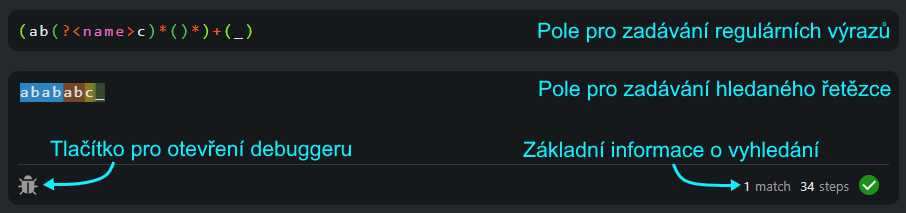
\includegraphics[width=0.85\textwidth]{Figures/appWindow.png}
	\caption{Úvodní uživatelské rozhraní}
	\label{fig:GeneralUI}
\end{figure}

\begin{figure}[!h]
	\centering
	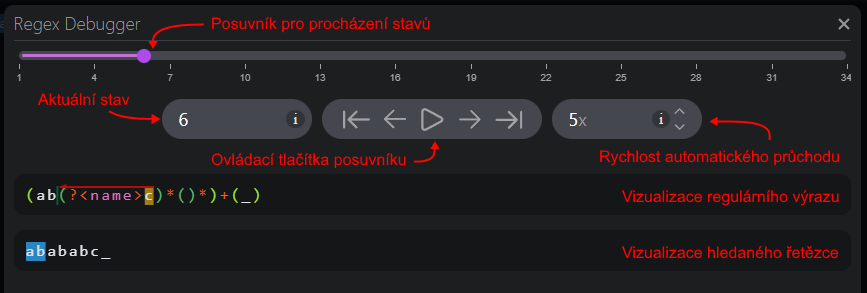
\includegraphics[width=0.85\textwidth]{Figures/appDebugger.png}
	\caption{Uživatelské rozhraní debuggeru}
	\label{fig:DebuggerUI}
\end{figure}

VSCode api zpřístupňuje využití css stylů, které má uživatel přímo nastavené ve svém prostředí.
Pokud je tedy webová stránka součástí VSCode prostředí, tak přejímám styly, které má uživatel přímo nastavené ve VSCode.
Součástí toho jsou, fonty, barvy, tmavý nebo světlý režim atd.
Jestliže má uživatel nastavený světlý režim, tak se také stránka automaticky přizpůsobí.

\section{VSCode rozšíření}

Samotné rozšíření je vyvíjeno, pro prostředí Visual Studio Code.
Výhodou tohoto prostředí, je lehká integrace webového rozhraní.
VSCode API samozřejmě zprostředkovává mnohem více možností, pro samotný vývoj rozšíření.

\subsection*{Integrace webového zobrazení}

Webové zobrazení, využívá tzv. webview, které zobrazí webovou stránku v omezeném režimu.
Omezení je například ve smyslu nutností explicitně povolit JavaScriptové kódy, spouštěné v samotném zobrazení.
Dalším problémem je načítání zdrojů.
Ty totiž nemohou být jednoduše brány z lokálních adresářů. 
Musí dojít ke konverzi adresy, na adresu podporovanou VSCode. 
K této změně, jsem použil vyhledání všech cest ke zdrojům.
Před tím než dojde k zobrazení webové stránky, je provedu konverzi na cestu podporovanou VSCode.

Zobrazení se může nacházet v několika částech prostředí.
Pro tuto aplikaci jsem zvolil, že se stránka zobrazí, v pravé části na polovinu obrazovky.
V budoucnu by, bylo možné přidat nastavení, aby si uživatel mohl zvolit, kde se bude okno aplikace zobrazovat.

Zobrazení aplikace lze také vyvolat najetím v textu na zadaný regulární výraz.
Po najetí se zobrazí tlačítko, které po jeho stisku otevře samotnou vizualizaci.
V té se bude již nacházet daný výraz, na který uživatel v textu najel.
Jelikož je aplikace integrována ve vývojovém prostředí, tak je podle mě výhodné mít jako přidanou hodnotu, využití větší interaktivity s prostředím.
VSCode API poskytuje možnost detekce pozice kurzoru myši, čehož jsem využil pro zmíněnou detekci.
Aby bylo možné rozpoznat, zda se na pozici v textu nachází syntaxe regulárního výrazu, musí proběhnout nějaké vyhodnocení textu.
Toto vyhodnocení probíhá pomocí specifického regulárního výrazu, který zjišťuje kontrolu zda se jedná o správný tvar.
Zmíněné řešení mě napadlo jako první, ale není ideální.
Vhodnější by bylo použít nějaký jazykový server, který by z daného textu automaticky rozpoznal, o jaký syntaktický prvek se jedná.

\subsection*{Možnosti nastavení rozšíření}

API pro VSCode nabízí možnost poskytnout nastavení pro rozšíření, které může uživatel měnit na základě svých preferencí.
Pro tuto aplikaci jsem přidal jednoduché a omezené možnosti nastavení.
První možnost nastavení se týká vypnutí a zapnutí funkce pro najetí na text, zmíněné v předchozí sekci.
Druhé nastavení udává, zda se má vytvářet pokaždé nové okno webového rozhraní, nebo se má překreslovat již existující.
Nastavení by mohlo existovat v budoucnu více, aby umožňovali uživatelům vyšší flexibilitu. 

\subsection*{Komunikace rozšíření a vizualizace}

Ke komunikaci VSCode s webview dochází pomocí zpráv.
Jedná se o komunikaci, která je předepsána pro VSCode API součástí jejich dokumentaci.
Komunikaci jsem se pokusil omezit na minimum, aby nedocházelo k přetížení aplikace.
Proto se posílají pouze zprávy, které souvisí s samotným rozšířením pro VSCode.
Například pokud dojde, k otevření výrazu z VSCode, tak musí dojít k jeho zaslání pomoci zprávy do webview.
Vizualizace se také může nacházet samostatně mimo kontext rozšíření, proto je automaticky posílání a přijímání zpráv vypnuté.

\section{Sestavení a spuštění projektu}

Pro vlastní sestavení aplikace je potřeba mít nainstalovaný NodeJS společně s NPM.
Při vývoji jsem používal NodeJS verze 20.9.0 a NPM verze 10.2.1.
Avšak pro vlastní sestavení, by měla stačit verze NodeJS 14.17 společně s NPM verzí 6.14.
Zároveň může být použité i novější verze. 
Pokud uživatel nemá NodeJS, lze jej nainstalovat ze stránky \textit{https://nodejs.org}, NPM je součástí instalace.
Lze použít i jiné balíčkové manažery místo NPM, ale v návodu na sestavení používám právě NPM.
Rozšíření bylo vyvíjeno pro VSCode verze 1.84.0, ale mělo by fungovat i na novějších verzích.

V příloze~\ref{sec:FileStructure}, je ukázaná částečná adresářová struktura projektu.
Instalace probíhá v následujících krocích:

\begin{enumerate}
	\item Pro instalaci všech externích závislostí, v kořenovém adresáři se použije příkaz \textbf{\textcolor{OliveGreen}{npm install}}
	\item K sestavení projektu slouží npm skript \textbf{\textcolor{OliveGreen}{npm run build}}
	\item Pro vytvoření instalačního souboru rozšíření se použije příkaz \textbf{\textcolor{OliveGreen}{npm run release}}
	\item Výsledný instalační soubory se nachází v \textit{/libraries/regex-visualizer-extension/release}, podle přílohy \ref{sec:FileStructure}
\end{enumerate}

Všechny potřebné soubory pro lokální spuštění ve webovém prohlížeči, se po přeložení nachází v adresáři \textit{/libraries/regex-visualization/dist}. 
Pro spuštění je poté potřeba mít jakýkoliv webový server, kvůli podpoře web workeru.

\subsection*{Výsledný instalační soubor}

Výsledným souborem pro VSCode rozšíření, je soubor s příponou \textit{.vsix}.
Tyto soubory slouží pro lokální instalaci rozšíření. 
Samotná rozšíření lze publikovat veřejně součástí VSCode marketplace, ale aktuálně jsem se rozhodl tuto aplikaci nepublikoval.
Pro získání \textit{vsix} souboru, slouží příkaz \textit{vsce}, který dokáže sjednotit všechny závislosti do jednoho výsledného souboru.

Pro instalaci rozšíření, lze použít příkazovou paletu od VSCode.
Tu lze otevřít přímo ve vývojovém prostředí, pomocí zkratky \textbf{Shift + Command + P} pro Mac, nebo pomocí \textbf{Ctrl + Shift + P} pro Windows/Linux.
Po otevření příkazové palety, stačí zadat příkaz \textit{Extensions: Install from VSIX}.
Poté se otevře průzkumník souborů, kde stačí otevřít zvolený \textit{vsix} soubor, který se nainstaluje.

\endinput